\documentclass{article}

\usepackage{graphicx}
\usepackage{tikz}
\usepackage{tikzsymbols}
\usetikzlibrary{calc,patterns,shapes.geometric}
\pagestyle{empty}
\usepackage[margin=0pt]{geometry}
\geometry{papersize={14in,12in}}

\def\centerarc[#1](#2)(#3:#4:#5){\draw[#1] ($(#2)+({#5*cos(#3)},{#5*sin(#3)})$) arc (#3:#4:#5);}

\begin{document}
	\begin{figure}
		\centering
		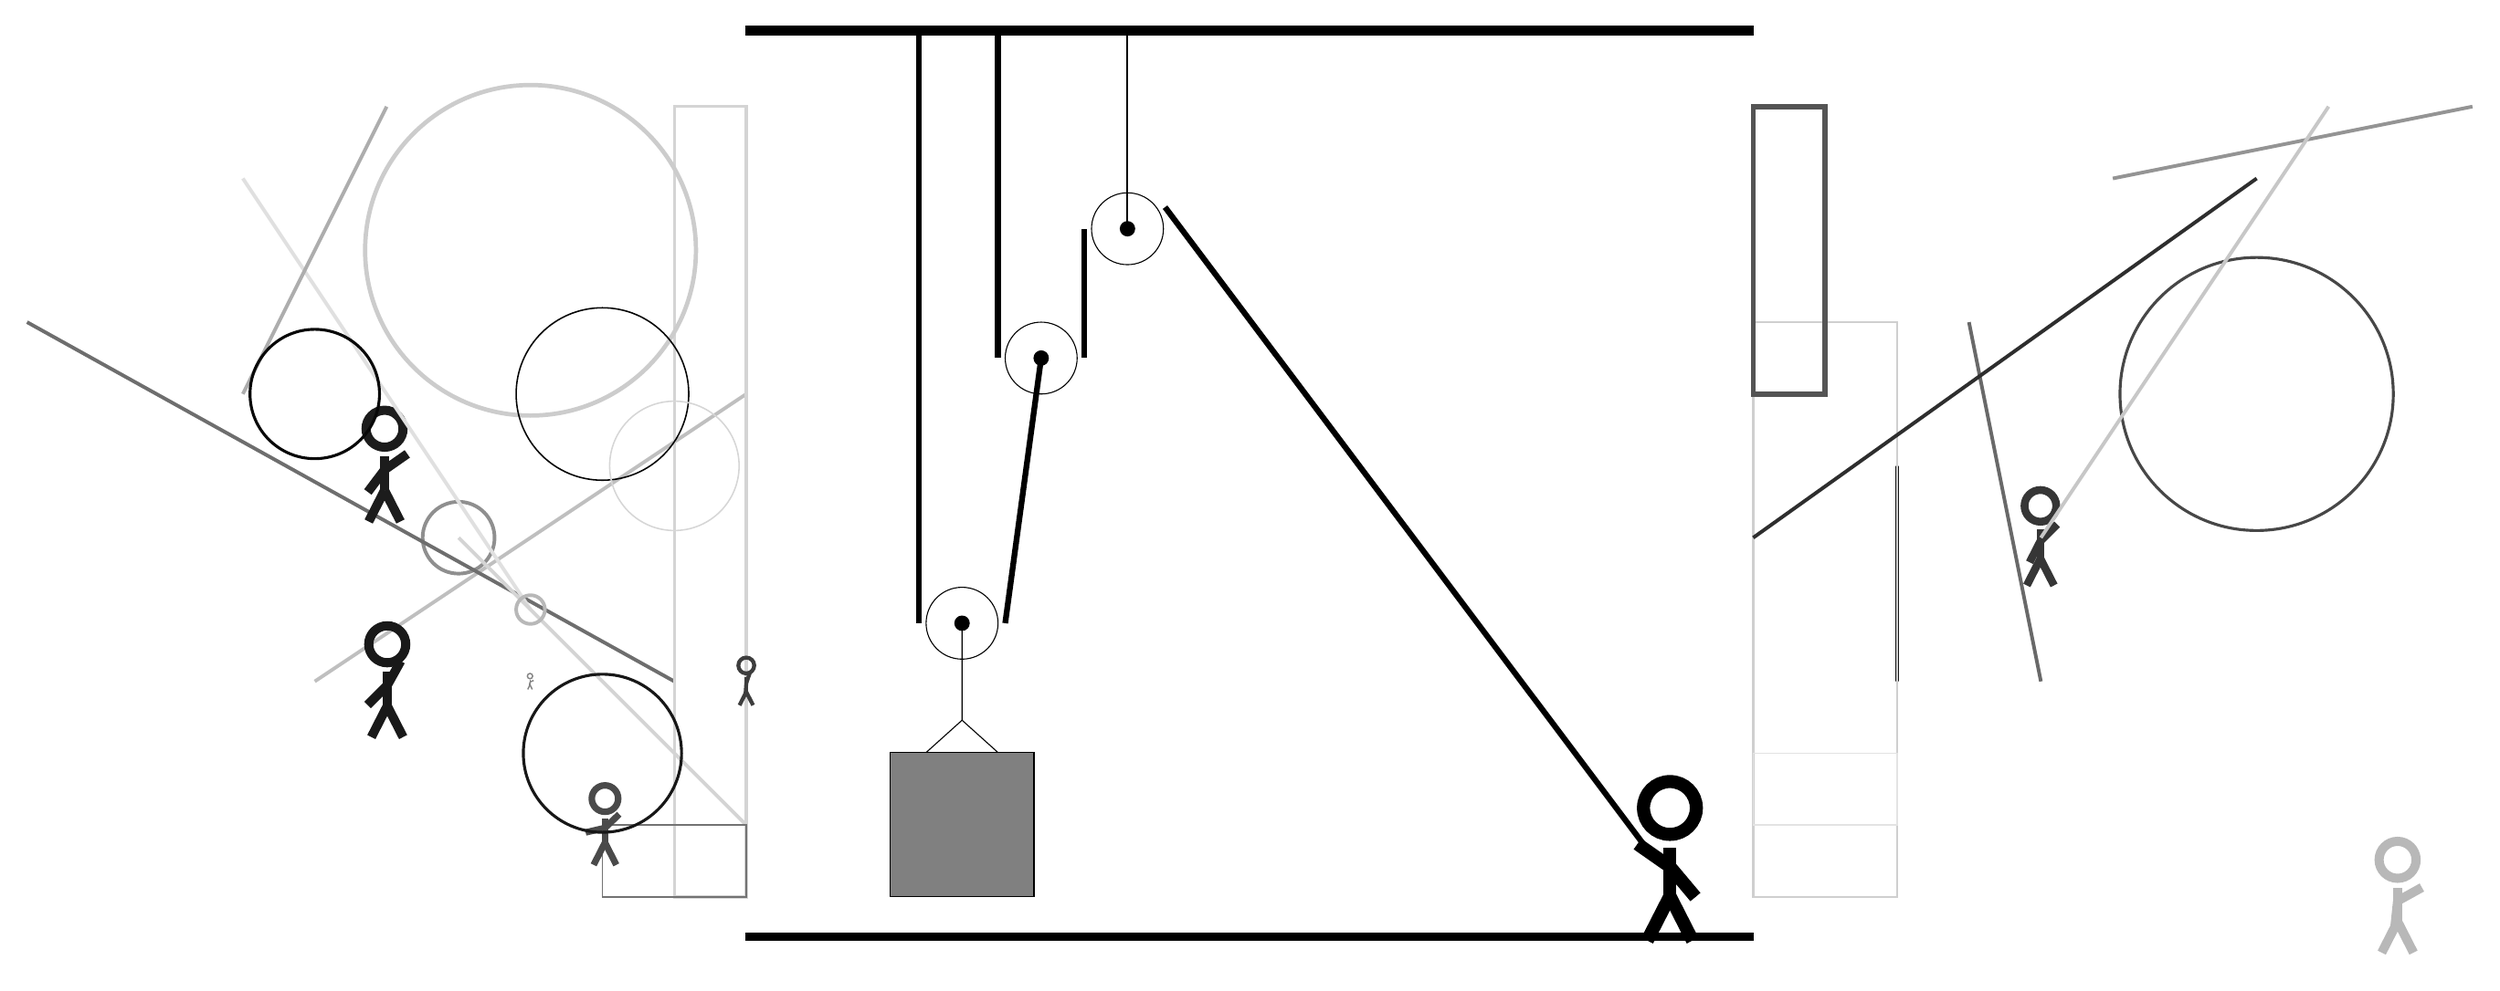
\begin{tikzpicture}
			%%%%% START %%%%%
			
			\draw[fill=black] (-2, 9) rectangle (12, 9.125);
			
			\draw (1, 0.81) circle (0.5);
			\draw[fill=black] (1, 0.81) circle (0.1);
			
			\draw (2.1, 4.5) circle (0.5);
			\draw[fill=black] (2.1, 4.5) circle (0.1);
			
			\draw (3.3, 6.3) circle (0.5);
			\draw[fill=black] (3.3, 6.3) circle (0.1);
			\draw[thick] (3.3, 6.3) -- (3.3, 9);
			
			\draw (1, 0.81) -- (1, -0.54) -- (0.5, -0.99) -- (1.5, -0.99) -- (1, -0.54);
			\draw[fill=black!50] (0, -0.99) rectangle (2, -2.99);
			
			\draw[line width=0.5mm, color=black!25](-2, 4) -- (-8, 0);
			
			\draw [line width=0.5mm, color=black!44](-6, 2) circle (0.5);
			\draw[line width=0.5mm, color=black!57](-3, 0) -- (-12, 5);
			\draw[line width=0.5mm, color=black!42](17, 7) -- (22, 8);
			
			\node[line width=0.3mm, color=black!89] at (-7, 3) {\Strichmaxerl[7][53][35]};
			
			\draw[line width=0.5mm, color=black!12](-5, 1) -- (-9, 7);
			
			\draw[line width=0.6mm, color=black!92] (14, 0) rectangle (14, 3);
			\node[line width=0.5mm, color=black!90] at (-7, 0) {\Strichmaxerl[7][45][61]};
			\draw[line width=0.4mm, color=black!17] (-2, -3) rectangle (-3, 8);
			\draw[line width=0.5mm, color=black!59](16, 0) -- (15, 5);
			
			\draw[line width=0.3mm, color=black!19] (14, 5) rectangle (12, -3);
			\node[line width=0.6mm, color=black!76] at (-2, 0) {\Strichmaxerl[3][86][71]};
			\draw[line width=0.2mm, color=black!11] (14, -2) rectangle (12, -1);
			
			\draw [line width=0.4mm, color=black!72](19, 4) circle (1.9);
			\draw[line width=0.5mm, color=black!32](-7, 8) -- (-9, 4);
			\draw[line width=0.5mm, color=black!17](-2, -2) -- (-6, 2);
			
			\draw [line width=0.5mm, color=black!28](-5, 1) circle (0.2);
			\node[line width=0.5mm, color=black!28] at (21, -3) {\Strichmaxerl[7][84][29]};
			\draw [line width=0.6mm, color=black!20](-5, 6) circle (2.3);
			\draw [line width=0.4mm, color=black!97](-8, 4) circle (0.9);
			\draw[line width=0.2mm, color=black!55] (-2, -3) rectangle (-4, -2);
			\node[line width=0.4mm, color=black!79] at (16, 2) {\Strichmaxerl[6][63][45]};
			
			\node[line width=0.3mm, color=black!49] at (-5, 0) {\Strichmaxerl[1][81][23]};
			\draw [line width=0.2mm, color=black!99](-4, 4) circle (1.2);
			\node[line width=0.6mm, color=black!71] at (-4, -2) {\Strichmaxerl[5][13][44]};
			\draw[line width=0.5mm, color=black!22](16, 2) -- (20, 8);
			\draw [line width=0.4mm, color=black!91](-4, -1) circle (1.1);
			\draw[line width=0.7mm, color=black!67] (13, 8) rectangle (12, 4);
			
			\draw[line width=0.5mm, color=black!82](12, 2) -- (19, 7);
			\draw [line width=0.2mm, color=black!16](-3, 3) circle (0.9);
			
			\draw[line width=0.8mm] (0.4, 9) -- (0.4, 0.81);
			\centerarc[line width=0.8mm](1, 0.81)(180:360:0.6);
			\draw[line width=0.8mm](1.6, 0.81) -- (2.1, 4.5);
			\draw[line width=0.8mm] (1.5, 9) -- (1.5, 4.5);
			\centerarc[line width=0.8mm](2.1, 4.5)(180:360:0.6);
			\draw[line width=0.8mm](2.7, 4.5) -- (2.7, 6.3);
			\centerarc[line width=0.8mm](3.3, 6.3)(30:180:0.6);
			\draw[line width=0.8mm] (3.822, 6.6) -- (10.5, -2.3);
			
			\node at (10.8, -2.5) {\Strichmaxerl[10][-35][-50]};
			
			\draw[fill=black] (-2, -3.5) rectangle (12, -3.6);
			
			%%%%% END %%%%%
		\end{tikzpicture}
	\end{figure}	
\end{document}